
\subsubsection{Sensitivity to Diffusion and Contaminant Inventory}

In the parametric sensitivity analysis discussed in section
\ref{sec:diffusivity}, it was shown that
The peak doses due to highly soluble, non-sorbing elements such as $I$ and $Cl$, 
are  proportional to the radionuclide inventory and 
largely directly proportional to the relative diffusivity. This can be seen for 
the cases of $^{129}I$ and $^{36}Cl$ in Figures \ref{fig:DCInvI129}, 
\ref{fig:DCInvI129MF}, \ref{fig:DCInvCl36} and \ref{fig:DCInvCl36MF}.

\begin{figure}[ht]
\centering
\begin{minipage}[b]{0.45\linewidth}

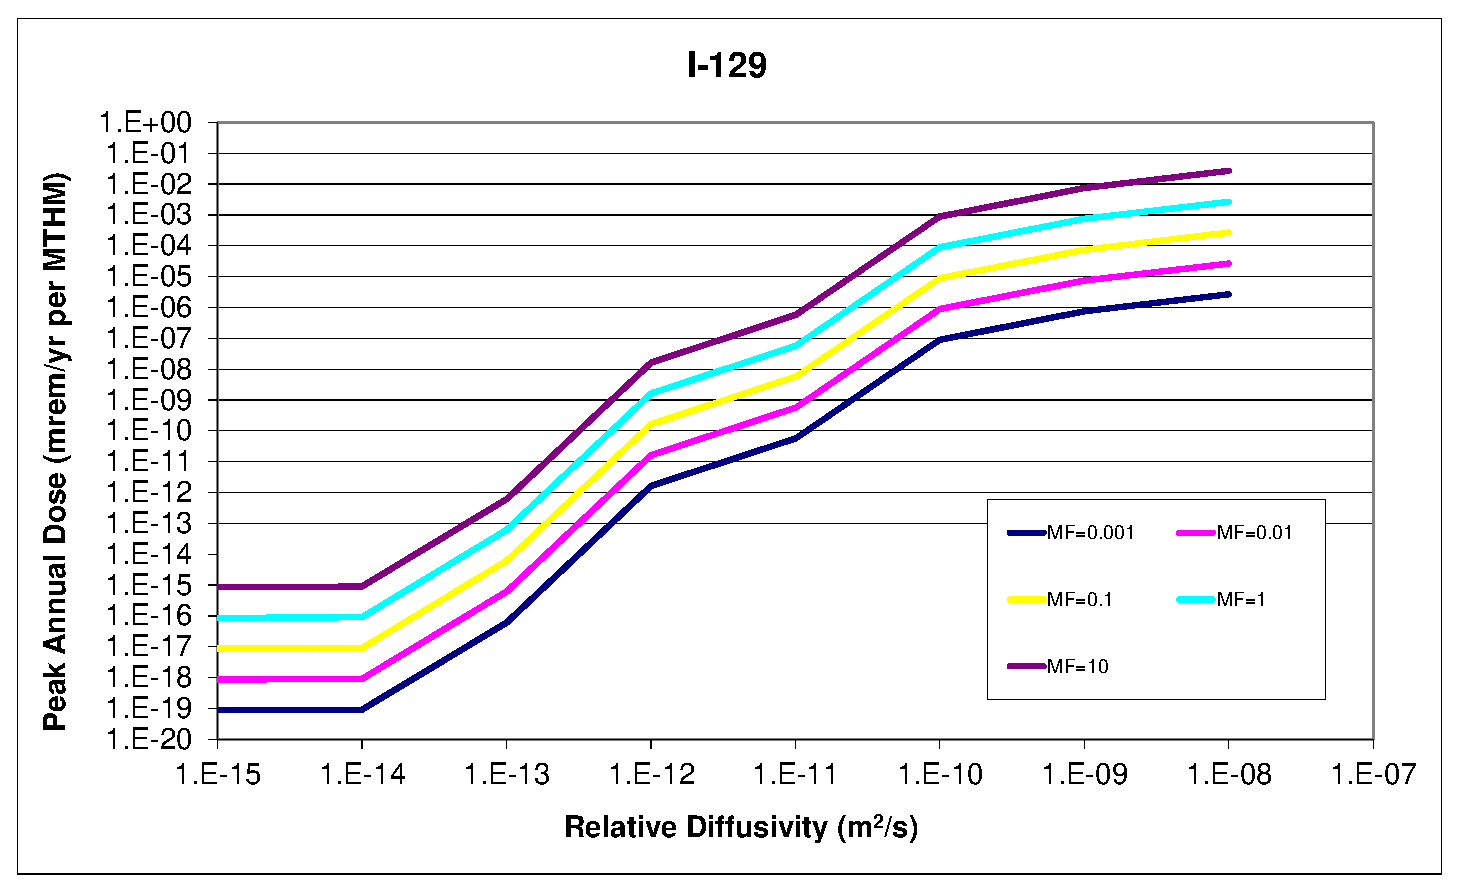
\includegraphics[width=\linewidth]{./chapters/nuclide_sensitivity/clay/DiffCoeffAndInvEBSFail/I-129.eps}
\caption{$^{129}I$ relative diffusivity sensitivity.}
\label{fig:DCInvI129}

\end{minipage}
\hspace{0.05\linewidth}
\begin{minipage}[b]{0.45\linewidth}

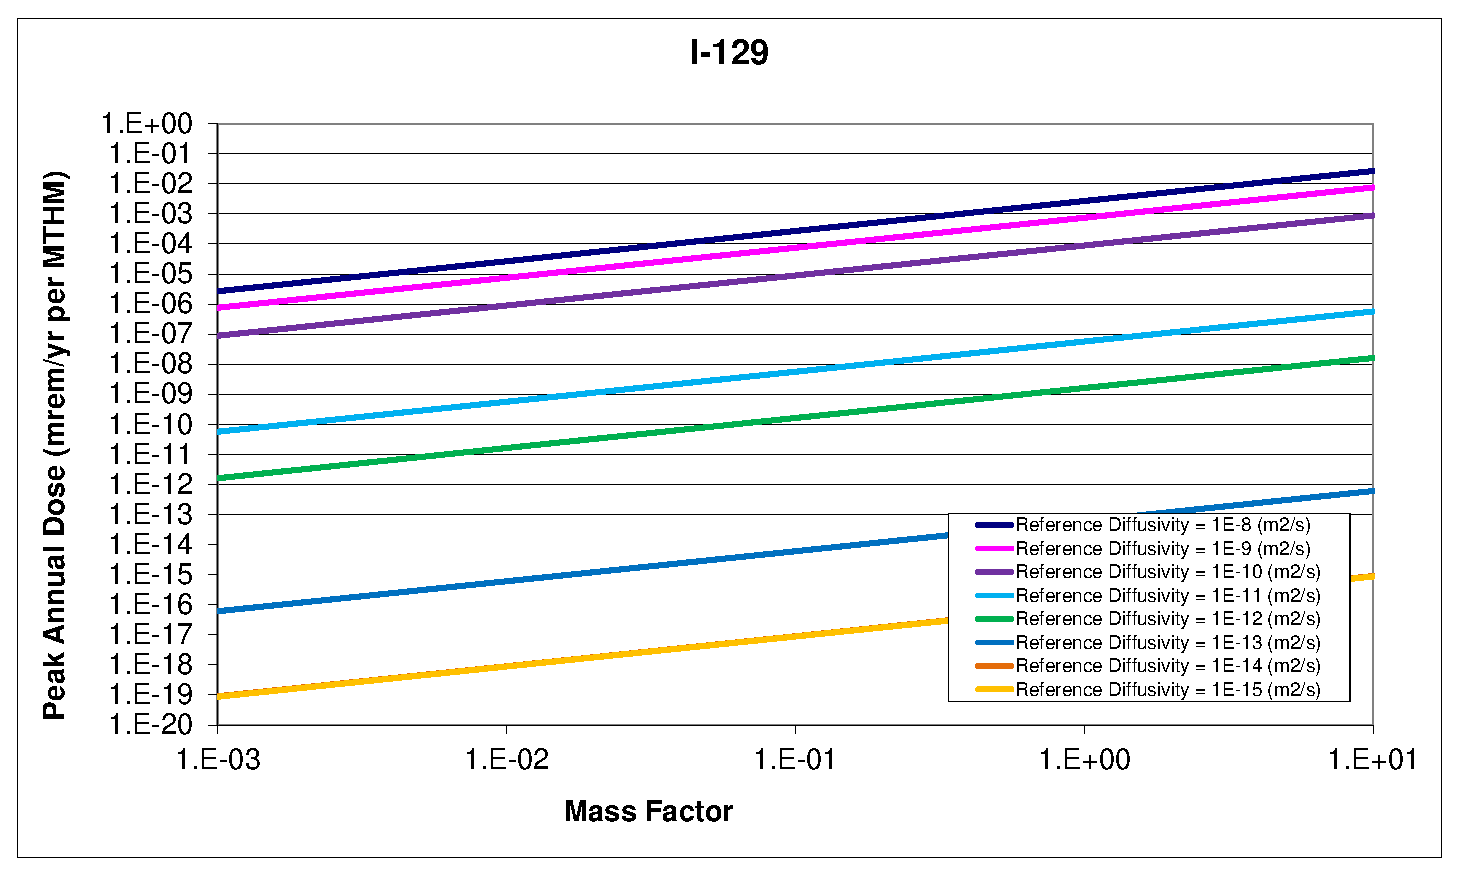
\includegraphics[width=\linewidth]{./chapters/nuclide_sensitivity/clay/DiffCoeffAndInvEBSFail/I-129-MF.eps}
\caption{$^{129}I$ mass factor sensitivity.}
\label{fig:DCInvI129MF}

\end{minipage}
\end{figure}

\begin{figure}[ht]
\begin{minipage}[b]{0.45\linewidth}

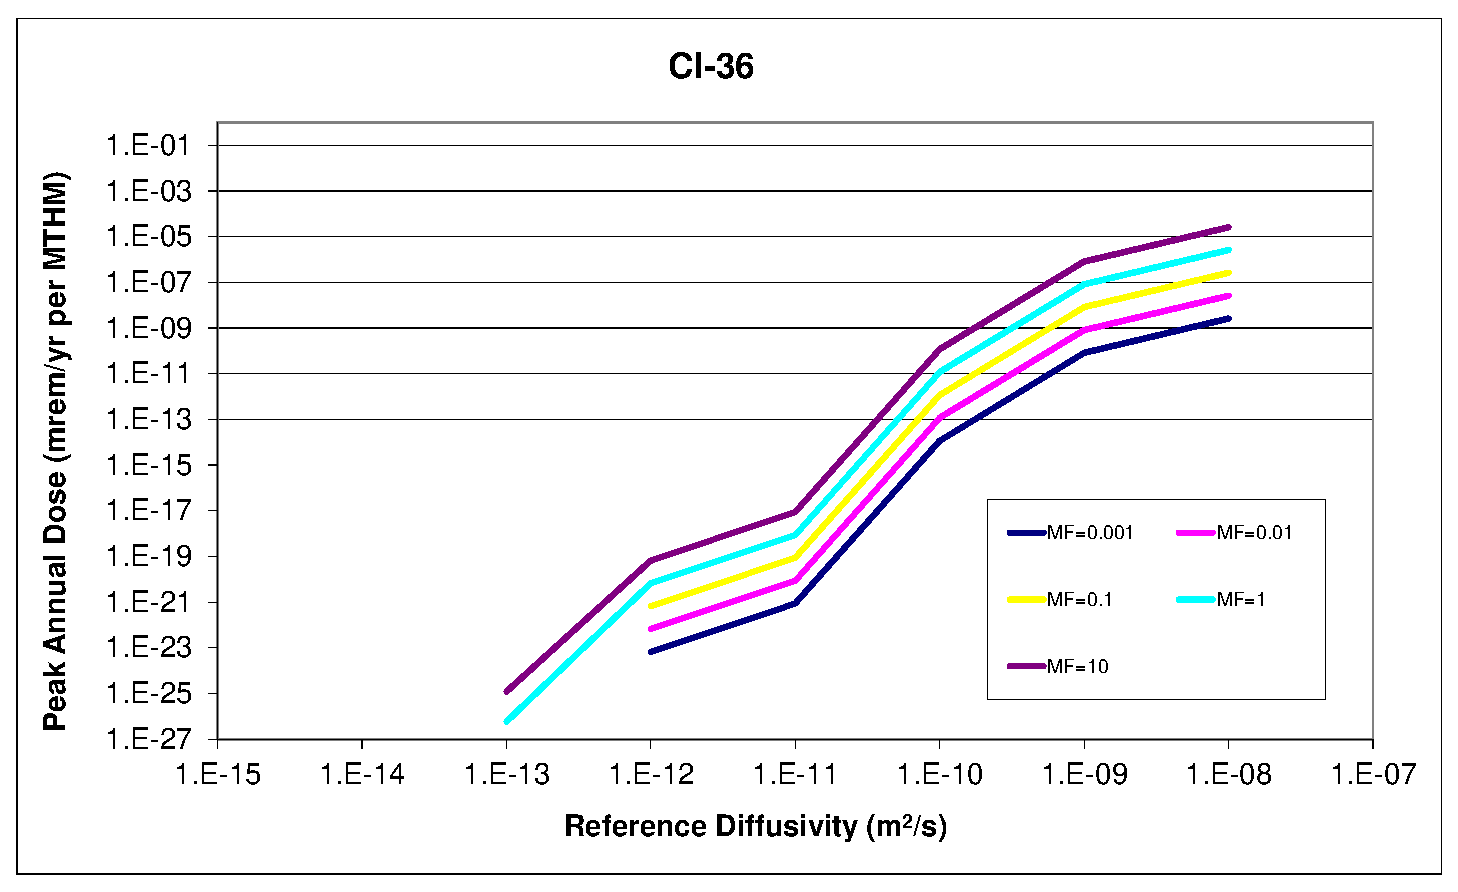
\includegraphics[width=\linewidth]{./chapters/nuclide_sensitivity/clay/DiffCoeffAndInvEBSFail/Cl-36.eps}
\caption{$^{36}Cl$ relative diffusivity sensitivity.}
\label{fig:DCInvCl36}

\end{minipage}
\hspace{0.05\linewidth}
\begin{minipage}[b]{0.45\linewidth}

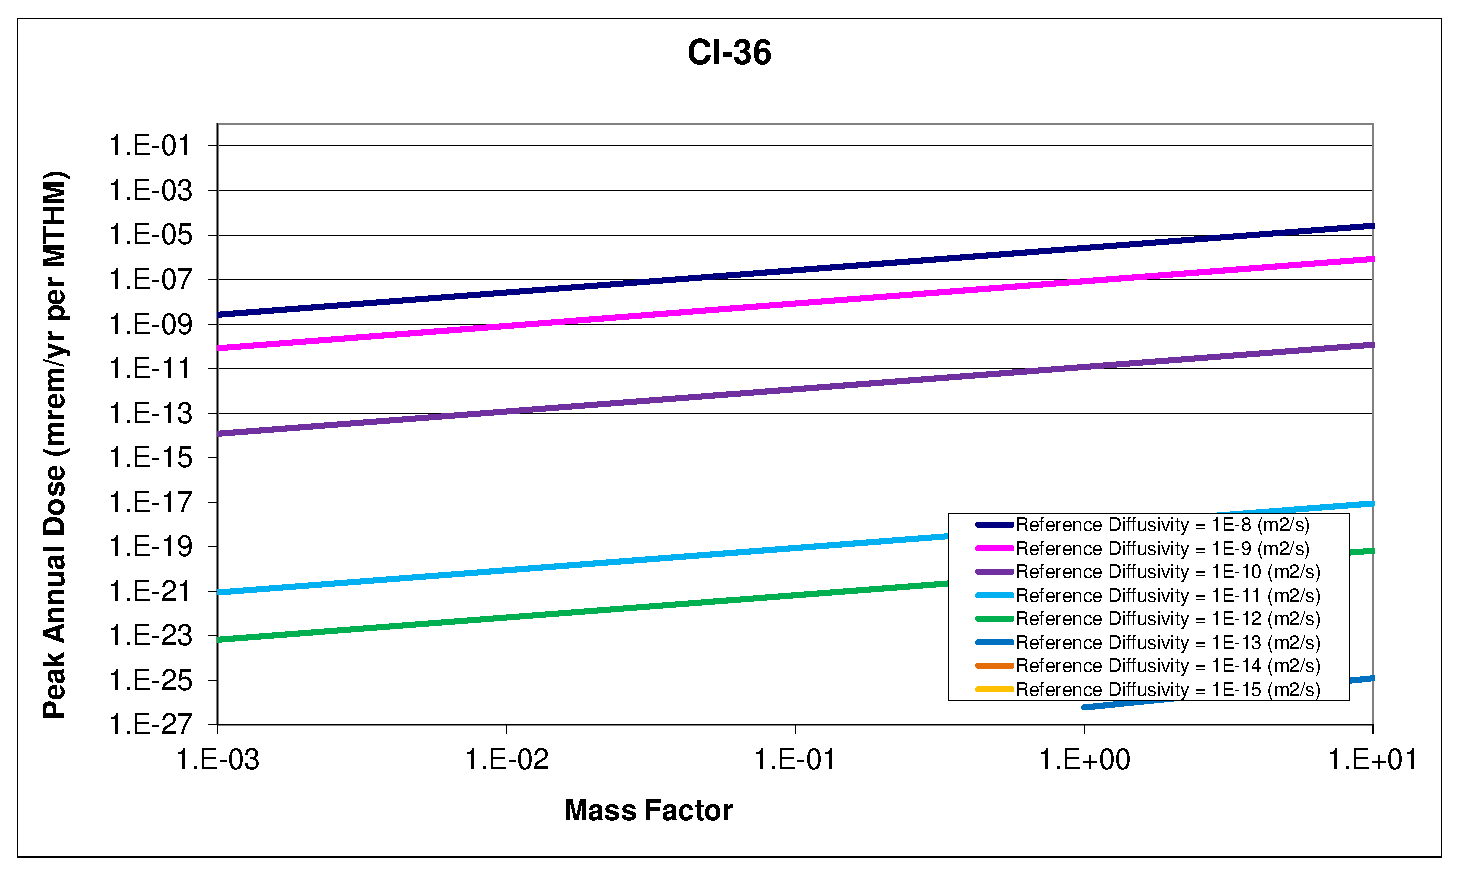
\includegraphics[width=\linewidth]{./chapters/nuclide_sensitivity/clay/DiffCoeffAndInvEBSFail/Cl-36-MF.eps}
\caption{$^{36}Cl$ mass factor sensitivity.}
\label{fig:DCInvCl36MF}

\end{minipage}
\end{figure}

Long lived $^{129}I$ and $^{36}Cl$ are assumed to have near complete solubility, 
so in Figures \ref{fig:DCInvI129} and \ref{fig:DCInvCl36}, the effect of a 
solubility limited attenuation regime is not seen. Even for very low 
diffusivities, the diffusion length of the far field is the primary barrier. In 
Figures \ref{fig:DCInvI129MF} and \ref{fig:DCInvCl36MF} it is clear that in the 
absence of solubility limitation and sorption, the peak dose is directly 
proportional to mass factor. 

Both $Cl$ and $I$ are soluble and non-sorbing. The amount of $^{129}I$ in the 
\gls{SNF} inventory is greater than the amount of $^{36}Cl$, so a difference in 
magnitudes are expected, however, the trends should be the same. Since the 
halflife of $^{36}Cl$, $3\times10^5[yr]$, is much shorter than the half life of 
$^{129}I$, $1.6\times10^7[yr]$, a stronger proportional dependence on mass 
factor is seen for $Cl$ due to its higher decay rate. 

With the exception of those dose-contributors assumed to be completely soluble, 
two regimes were visible in the results of this analysis. In low diffusion 
coefficient regime, the diffusive pathway through the homogeneous permeable 
porous medium in the far field continues to be a  dominant barrier to nuclide 
release for normal (non-intrusive) repository conditions. 

In the second regime, for very high diffusion coefficients, the effects of 
additional attenuation phenomena in the natural system can be seen.  The 
dependence of peak annual dose on mass factor was consistently directly 
proportional for all isotopic groups.

The peak doses due to solubility limited, sorbing elements such as $Np$ and 
$Tc$ demonstrate two major regimes. In the first regime, for 
low values of mass factor, the mean of the peak annual dose rates is directly 
proportional to both reference diffusivity and mass factor.  For higher values 
of mass factor, the sensitivity to reference diffusivity and mass factor are 
both attenuated at higher values.  The attenuation in these regimes 
is due to natural system attenuation, most notably, sorption.

$^{237}Np$ and $^{99}Tc$ exhibit a strong proportional relationship 
between diffusivity and dose in Figures \ref{fig:DCInvTc99} and 
\ref{fig:DCInvNp237}. This relationship is muted as diffusivity 
increases. Both are directly proportional to mass factor until they reach the 
point of attenuation by their solubility limits, as can be seen in 
Figures \ref{fig:DCInvTc99MF} and \ref{fig:DCInvNp237MF}.

\begin{figure}[ht!]
\centering
\begin{minipage}[b]{0.45\linewidth}
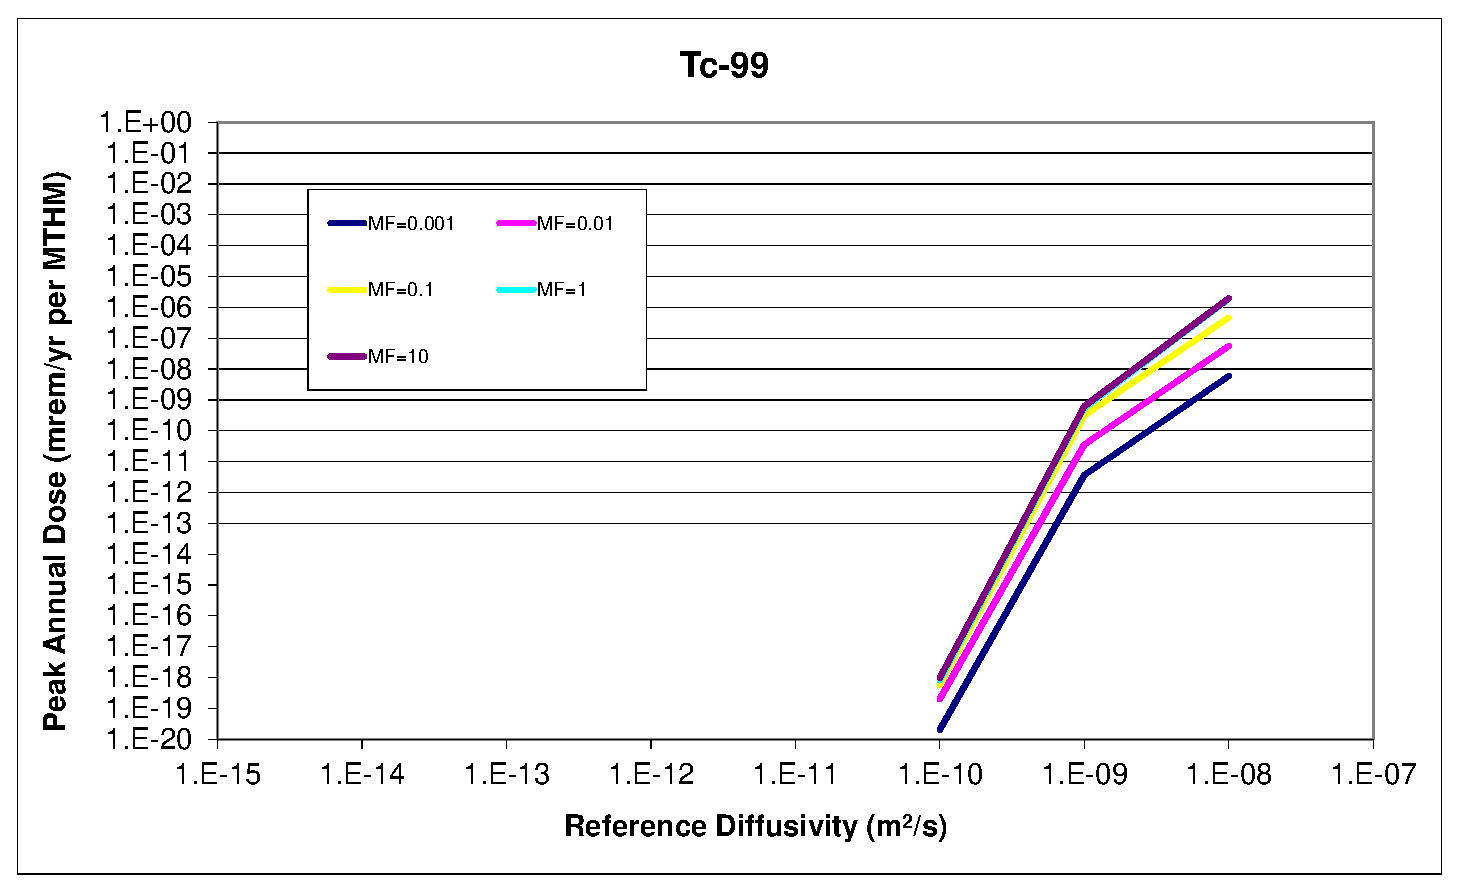
\includegraphics[width=\linewidth]{./chapters/nuclide_sensitivity/clay/DiffCoeffAndInvEBSFail/Tc-99.eps}
\caption{$^{99}Tc$ relative diffusivity sensitivity.} 
\label{fig:DCInvTc99}

\end{minipage}
\hspace{0.05\linewidth}
\begin{minipage}[b]{0.45\linewidth}

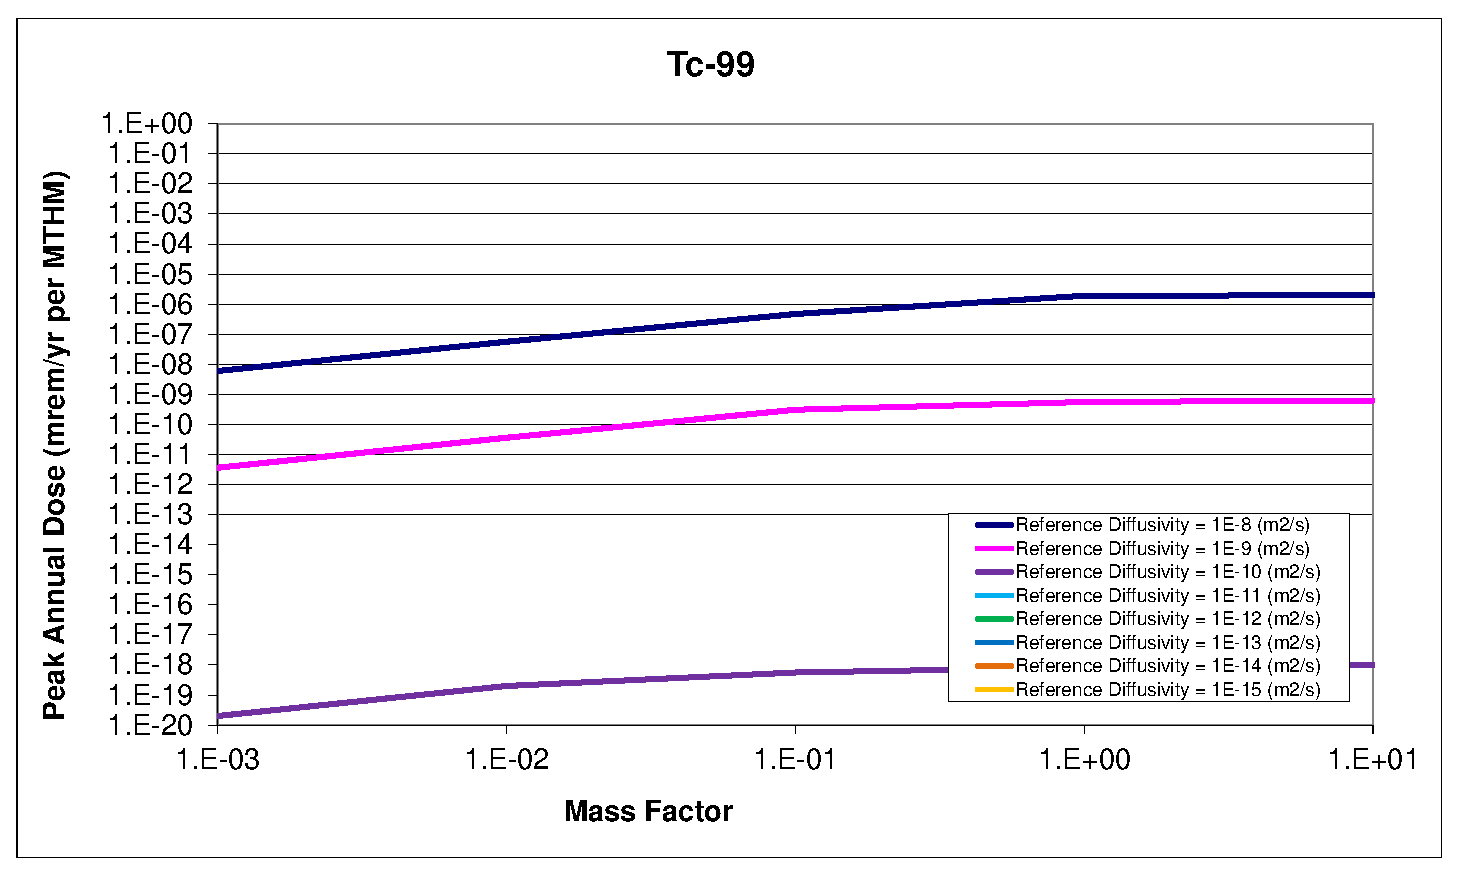
\includegraphics[width=\linewidth]{./chapters/nuclide_sensitivity/clay/DiffCoeffAndInvEBSFail/Tc-99-MF.eps}
\caption{$^{99}Tc$ mass factor sensitivity.}
\label{fig:DCInvTc99MF}

\end{minipage}
\end{figure}
\begin{figure}[ht]
\begin{minipage}[b]{0.45\linewidth}

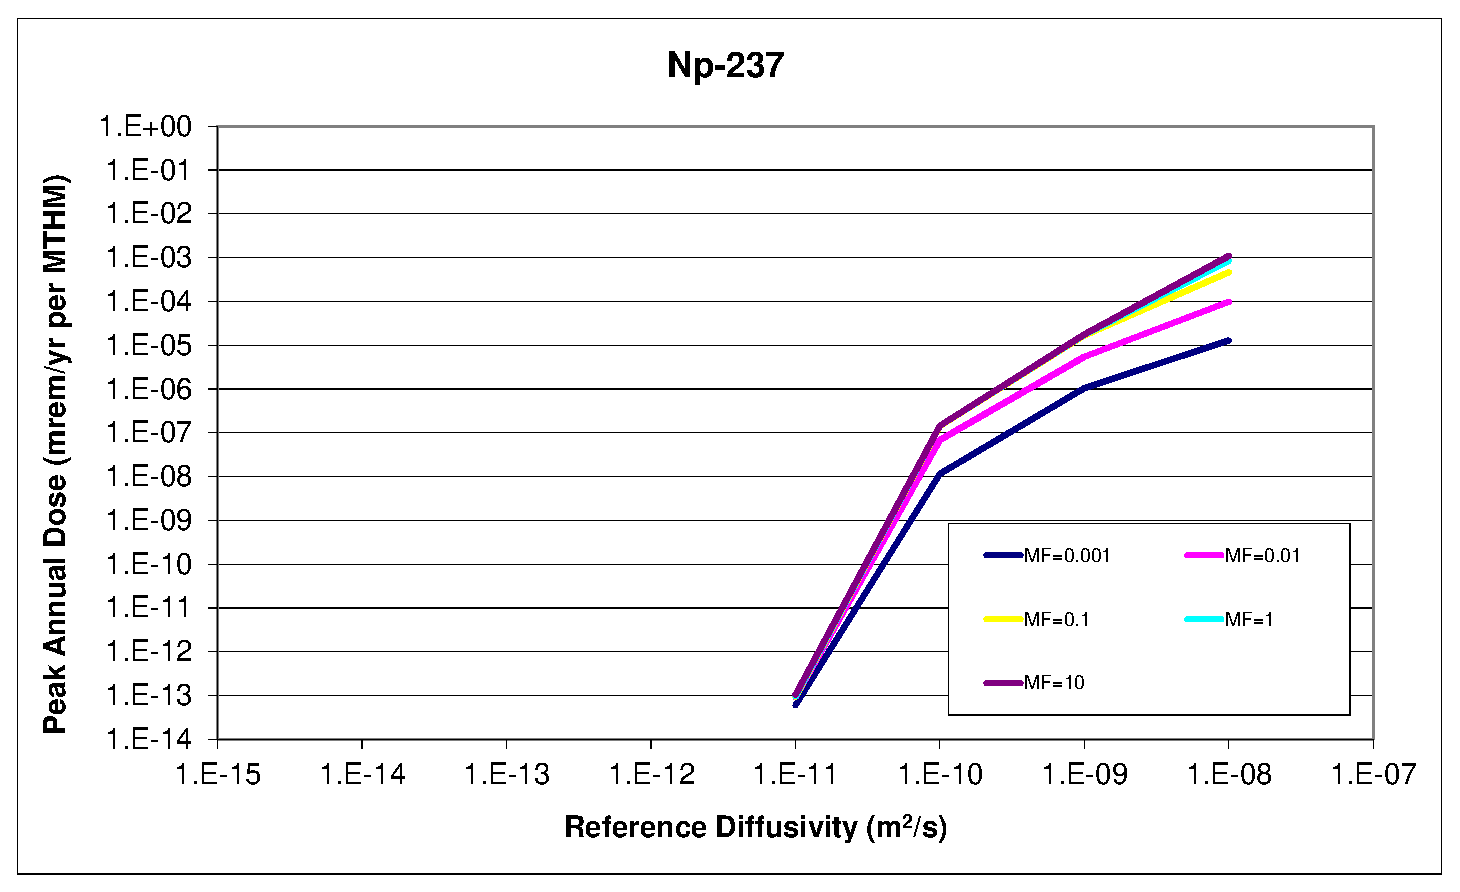
\includegraphics[width=\linewidth]{./chapters/nuclide_sensitivity/clay/DiffCoeffAndInvEBSFail/Np-237.eps}
\caption{$^{237}Np$ relative diffusivity sensitivity.} 
\label{fig:DCInvNp237}

\end{minipage}
\hspace{0.05\linewidth}
\begin{minipage}[b]{0.45\linewidth}

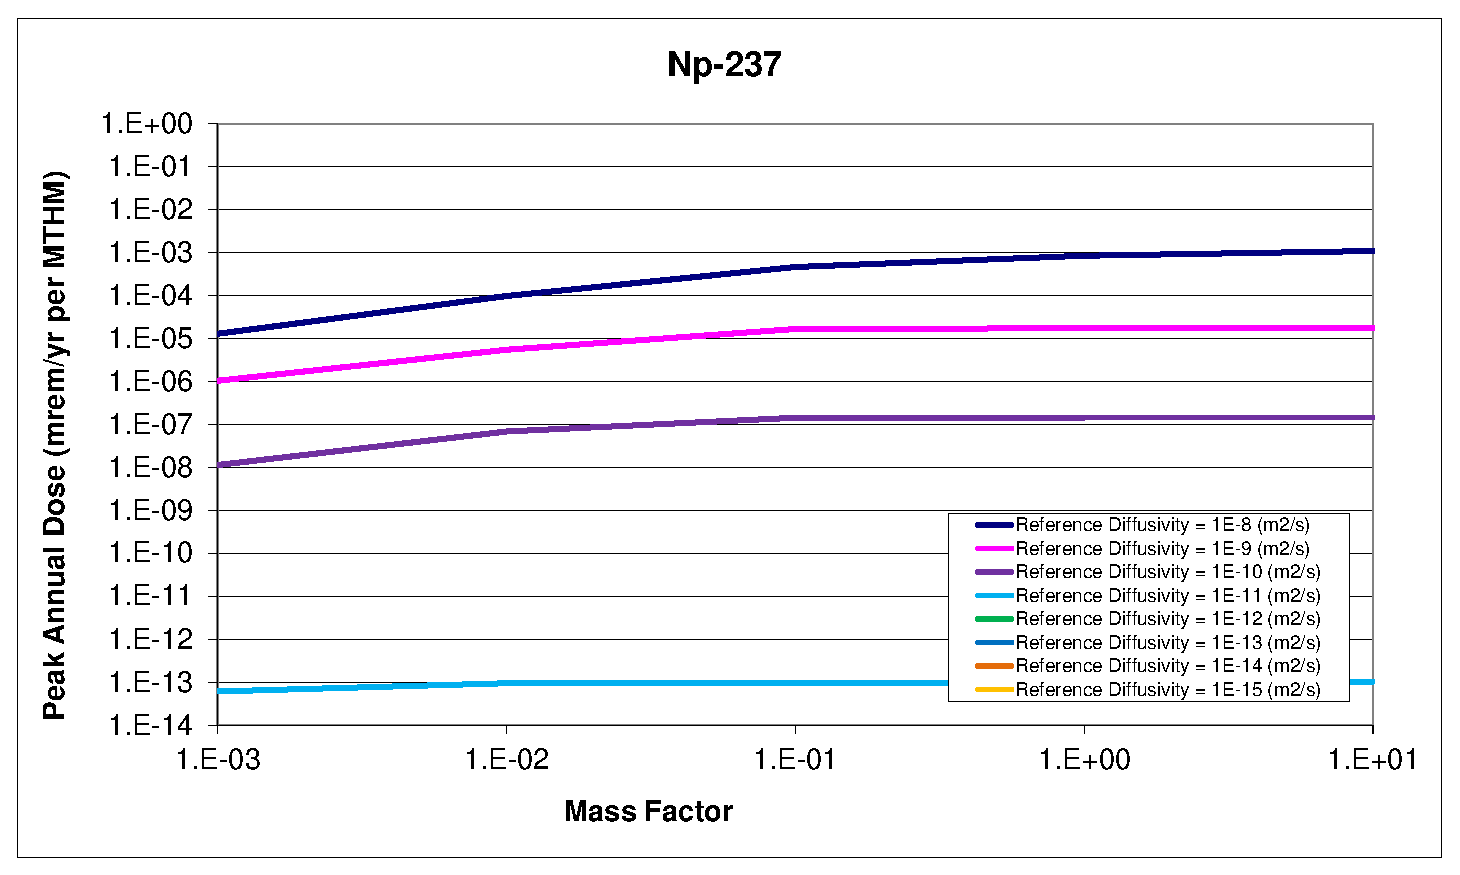
\includegraphics[width=\linewidth]{./chapters/nuclide_sensitivity/clay/DiffCoeffAndInvEBSFail/Np-237-MF.eps}
\caption{$^{237}Np$ mass factor sensitivity.}
\label{fig:DCInvNp237MF}

\end{minipage}
\end{figure}


\clearpage


